\chapter{Design}
  The following sections will cover the modularisation and the modules themselves. Each module will be described in detail which data it takes and which it will provide as well as the functionalities of it. Additional to the modules the specification will also give information on the different data that will be created and stored persistent.

  The whole project will be based on packet loss, but it should be designed to use other methods as well like the signal strength to perform a position detection.

  The UML Diagrams that are shown here are reduced to the important functions. This is because the Qt framework needs a lot of small functions that are not doing much but are needed to react on actions like hitting a button or clicking on a menu item.

  All modules that are marked as optional are implemented if there is some spare time or other modules can be done faster than planned.

  \section{Modularisation}
  \label{sec:design:modularisation}
   \begin{figure}[h]
    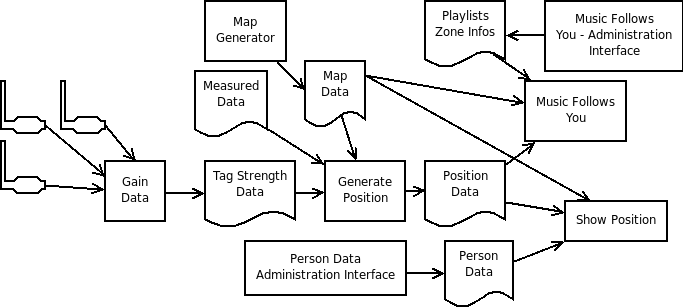
\includegraphics[scale=0.6]{Diagrams/projectStructure.png}
    \caption{Project modularisation and flow of data}
    \label{fg:projectModularization}
   \end{figure}

   Like it is shown in figure \ref{fg:projectModularization} the project will be separated into several functional modules. Those modules will be described in the following sections. Additional to the shown modules the following will also cover the changes that needed to be made to the firmware. The sections will also cover the data that will be stored persistent (Measurement, playlists, zone information, map and person data).

%%%%%%%%%%%%%%%%%%%%%%%%
%%%%%%  FIRMWARE  %%%%%%
%%%%%%%%%%%%%%%%%%%%%%%%
  \section{Firmware}
   \label{sec:design:firmware}
   The firmware of the OpenBeacon nodes needs some little adjustments in its functionalities. The following list will show which functionalities are already implemented and which shall be implemented additional to the existent.

   \subsection{Current functionalities}
    \begin{enumerate}
     \item Reading the whole configuration at once.
     \item Display a help screen. A functionality which is good if a user wants to interact but useless if a program wants to interact automatically with the node.
     \item Setting the id of the reader. This setting is used to differ between multiple nodes attached to one computer.
     \item Setting the cache (FIFO) size in seconds, the larger the cache size is the more packages will be received and the more accurate the node will get. But if the time for the cache is too high even small disturbances, like a small object, will have a big effect on the accuracy.
     \item Setting the node to receive only, in which it will not send any packages to the CCC Sputnik RFID tag.
     \item Setting the transmission power level of the OpenBeacon node to one of the 4 levels (1=0x00, 2=0x55, 3=0xAA, 4=0xFF).
     \item Saving all changes that were made.
    \end{enumerate}

   \subsection{Needed functionalities}
    \begin{enumerate}
     \item Reading only the id of the node. This functionality will lower the effort which is needed to parse for the id if the whole configuration will be read, it will also lower the amount of data that will be received. This configuration information is needed to identify each of the nodes connected to the computer
     \item Reading only the FIFO cache lifetime is not directly needed by the project but it will give the node a consistent interface.
     \item Reading the current power level on which the node is working. (0=receive only mode, 1=0x00, 2=0x55, 3=0xAA, 4=0xFF)
     \item Reading only the uptime of the node will be used for statistics only.
     \item Reading only the channel of the node. (Again this is not used directly by the project but will keep the interface consistent)
    \end{enumerate}

%%%%%%%%%%%%%%%%%%%%%%%%
%%%%%%  OBConfig  %%%%%%
%%%%%%%%%%%%%%%%%%%%%%%
  \section{OpenBeacon Configurator}
  \label{sec:design:OBConfig}
   The OpenBeacon Configurator is a simple GUI, which will be used to configure the OpenBeacon nodes as easy as possible.

   \subsection{Functionalities}
    \begin{itemize}
     \item Configuration of OpenBeacon nodes.
     \item Read information from OpenBeacon node.
     \item Write information to OpenBeacon node.
     \item Persistent saving of the information on the OpenBeacon node.
    \end{itemize}

   \subsection{UML Class Diagram}
    \begin{staticFigure}
     \centering
     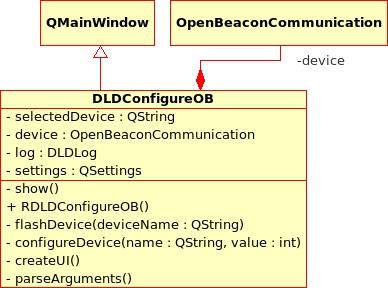
\includegraphics[scale=0.7]{UMLDiagrams/dldConfigureOB.png}
     \caption{UML class diagram of the OpenBeacon Configurator}
     \label{fg:projectModularization:OBConfigUML}
    \end{staticFigure}

%%%%%%%%%%%%%%%%%%%%%%%%%%%%%%%%
%%%%%%  GAIN DATA DAEMON  %%%%%%
%%%%%%%%%%%%%%%%%%%%%%%%%%%%%%%%
  \section{Gain data Daemon}
   \label{sec:design:gainDaemon}
    The gain data daemon communicates with all connected OpenBeacon nodes, it has a configuration file which describes each of the connected nodes. This description is not based on their device nodes in the system, but on their configured id's because the devices may change when they are plugged into the computer in a different order than the first time. The information which is gained will be provided to interested parties through a D-Bus or SSL connection. The provided strength is calculated with the following formula: $\textrm{strength} = \frac{\textrm{power level}}{85} * 10 + \left(\textrm{maximum packages} - \textrm{packet loss}\right)$

    A gain data daemon has the ability to watch over more than one OpenBeacon node at once. 

   \subsection{Functionalities}
    \begin{itemize}
     \item Read information from several OpenBeacon nodes.
     \item Providing the strength data of several tags.
     \item Provide which maximum packet loss is set.
    \end{itemize}

   \subsection{Incoming data}
    \begin{itemize}
     \item The incoming data to the gain data daemon consists of the raw data (for more information see listing \ref{lst:cuCommand}) of each of the OpenBeacon nodes.
     \item The settings of the several OpenBeacon nodes.
     \item The configuration of the data gain daemon.
    \end{itemize}

   \subsection{Outgoing data}
    \begin{itemize}
     \item One package for each update including the tag id, its strengths. (tagId$|$ nodeId1=strength1$|$nodeId2=strength2$|$\dots)
     \item A list of all tags that were in reach of the node(s)
     \item A list of all the connected node(s)
    \end{itemize}

   \subsection{UML Class Diagram}
    \begin{staticFigure}
     \centering
     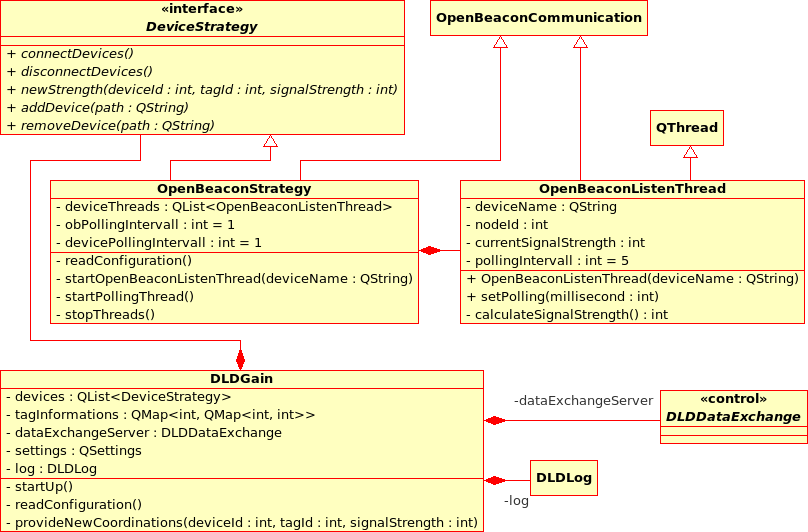
\includegraphics[scale=0.45]{UMLDiagrams/dldGain.png}
     \caption{UML class diagram of the Gain Data Daemon}
     \label{fg:projectModularization:gainDataDaemon}
    \end{staticFigure}

%%%%%%%%%%%%%%%%%%%%%%%%%%%%%%%%
%%%%%%   MEASURED DATA    %%%%%%
%%%%%%%%%%%%%%%%%%%%%%%%%%%%%%%%
  \section{Measured data}
   \label{sec:design:measuredData}
   The measured data is a fixed data block. The data that will be stored is based on a measurement that will be done by the developer itself and will cover a table of metric ranges compared to the packet loss or signal strength of the hardware. This data will be used by the generate position daemon described in section \ref{sec:design:generatePositionDaemon}. The data has to be gained once during the whole use of the project and it only will be changed if the project shows some failures in measurement or if the surrounding environment will change dramatically so the data does not correspond any more.

   \subsection{Functionalities}
    The measured data has no functionality for itself, it will only be used by other daemons to do a proper position detection.

   \subsection{Incoming data}
    \begin{itemize}
     \item packet data from data gain daemon (see section \ref{sec:design:gainDaemon})
     \item metric data from the person who will do the measurement
    \end{itemize}

   \subsection{Outgoing data}
    A table which will compare packet loss and power level to metric units. Each row of the table has to store the following data and each table needs to store the maximum of packets that could be received.
    \begin{itemize}
     \item power level
     \item packets received
     \item approximately distance in centimetre
    \end{itemize}

%%%%%%%%%%%%%%%%%%%%%%%%%%%%%%%%%%%%%%%%%%%%
%%%%%%   MAP GENERATION APPLICATION   %%%%%%
%%%%%%%%%%%%%%%%%%%%%%%%%%%%%%%%%%%%%%%%%%%%
  \section{Optional application - Map generation application}
   \label{sec:design:createMapAppl}
   This application will be used to create map files. Those map files will be used for displaying the position of a person (see section \ref{sec:design:showPosition}) as well as at the daemon that will generate the position data (see section \ref{sec:design:generatePositionDaemon}). The map data will consist of two files, a picture which will show the map itself, and a description file which will hold information upon the map. This information contains the zones and their names, the size of the map, a meter pixel correspondent, the name of the map. Zones are special regions on the map which can be used by special applications.

   \subsection{Functionalities}
    \begin{itemize}
     \item Open favourite drawing tool for map drawing
     \item Show picture of map and create information regarding this map
     \item Define different zones through polygons that are built with the help of the image file
     \item Save map data in a map package (see \ref{sec:design:map})
     \item Load data from a map package
     \item Change data from a map package
    \end{itemize}

   \subsection{Incoming data}
    \begin{itemize}
     \item map image from painting tool
     \item information given by the user
    \end{itemize}

   \subsection{Outgoing data}
    \begin{itemize}
     \item map package (see \ref{sec:design:map})
    \end{itemize}

   \subsection{UML Class Diagram}
    \begin{staticFigure}
     \centering
     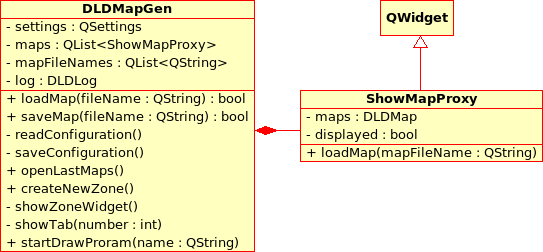
\includegraphics[scale=0.6]{UMLDiagrams/dldMapGen.png}
     \caption{UML class diagram of the Map generation application}
     \label{fg:projectModularization:mapGen}
    \end{staticFigure}

%%%%%%%%%%%%%%%%%%%%%%%%%%%%%%%%%%%%%%
%%%%%%   GENERATE POSITION DAEMON    %%%%%%
%%%%%%%%%%%%%%%%%%%%%%%%%%%%%%%%%%%%%%
  \section{Generate position daemon}
   \label{sec:design:generatePositionDaemon}
    The generate position daemon takes the information provided by the data gain daemon (see section \ref{sec:design:gainDaemon}) and creates the position data by triangulation like described in section \ref{sec:research:math}.

    The location detection will be based on the power level and the packet loss of the arriving packages. Three packages, each from a different node are needed to determine a position of a tag. The gained position will then be provided by sending it to a specific position. The position for each tag will be in packet loss not in any standard metric units.

    The gained position then will be either provided in a raw format or with the help of the measured data it will calculate an absolute position regarding a map (see \ref{sec:design:map}).

   \subsection{Functionalities}
    \begin{itemize}
     \item Check if all nodes are using the same packet loss parameters.
     \item Performing a mathematical position detection based on the strength.
     \item provide data in relative position
     \item provide data in absolute map position
     \item provide zone information of the tags
    \end{itemize}

   \subsection{Incoming data}
    \begin{itemize}
     \item strength data from the gain daemon (see outgoing data from section \ref{sec:design:gainDaemon})
     \item map package (see \ref{sec:design:map})
     \item measured data (see section \ref{sec:design:measuredData})
    \end{itemize}

   \subsection{Outgoing data}
    \begin{itemize}
     \item relative position data for each tag id
     \item absolute position data for each tag id
     \item zone information for each tag id
    \end{itemize}

   \subsection{UML Class Diagram}
    \begin{staticFigure}
     \centering
     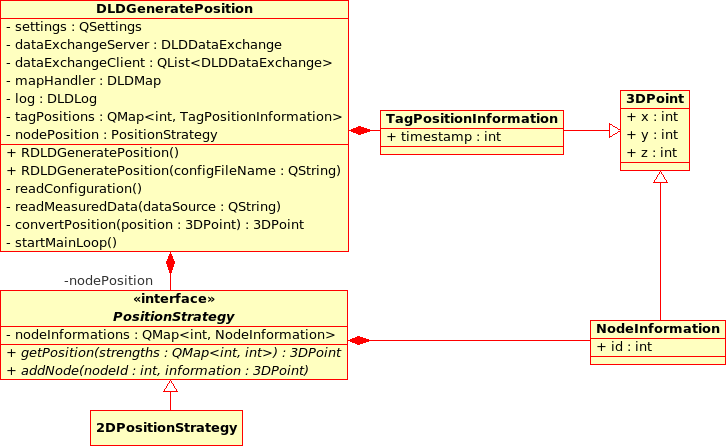
\includegraphics[scale=0.55]{UMLDiagrams/dldGeneratePosition.png}
     \caption{UML class diagram of the generate position daemon}
     \label{fg:projectModularization:generatePosition}
    \end{staticFigure}

%%%%%%%%%%%%%%%%%%%%%%%%%%%%%%%%%%%%%%%%%%%%%%%%%%
%%%%%% PERSON DATA ADMINISTRATION INTERFACE %%%%%%
%%%%%%%%%%%%%%%%%%%%%%%%%%%%%%%%%%%%%%%%%%%%%%%%%%
  \section{Person data administration interface}
   \label{sec:design:personDataAdmin}
   This application will be used to easily add information data regarding each person on the system. It will store basic information as well as the id of the tag the person is using.

   This application should be as flexible as possible and should not be fixed on persons. This will offer the possibility to use this application for objects as well.

   \subsection{Functionalities}
    \begin{itemize}
     \item Change the currently used database
     \item Create new entries in the database
     \item Change entries in the database
     \item Delete entries from database
     \item Show entries in database
    \end{itemize}

   \subsection{Incoming data}
    \begin{itemize}
     \item Information from administrator regarding the person
    \end{itemize}

   \subsection{Outgoing data}
    \begin{itemize}
     \item Persistent data stored in database.
    \end{itemize}

   \subsection{UML Class Diagram}
    \begin{staticFigure}
     \centering
     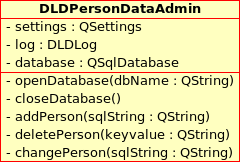
\includegraphics[scale=0.6]{UMLDiagrams/dldPersonDataAdmin.png}
     \caption{UML class diagram of the Person data administration interface}
     \label{fg:projectModularization:personDataAdmin}
    \end{staticFigure}

%%%%%%%%%%%%%%%%%%%%%%%%%%%%%%%%%%%%%%%%%%%%
%%%%%%   SHOW POSITION OF A PERSON    %%%%%%
%%%%%%%%%%%%%%%%%%%%%%%%%%%%%%%%%%%%%%%%%%%%
  \section{Show position of a person}
   \label{sec:design:showPosition}
   This application will show the position of a tag on a map. The tag id will be assigned to a person. The information to a person will be collected from a person database where needed information upon the person will be stored. This application should be as flexible as possible, therefore the information that will be displayed should not be fixed but should be variable. This will enable the application to be used for a different set of uses.

   \subsection{Functionalities}
    \begin{itemize}
     \item Select data source for assignment
     \item Assign tag id to person
     \item Display the position of a person on a map
     \item Select persons on the map
     \item Display information of visible persons
    \end{itemize}

   \subsection{Optional functionalities}
    \begin{itemize}
     \item Display short information in a fancy way, like a box next to the person that moves with it
     \item Mouse over selection of a person
     \item Display more than one map at once (in a tab view)
    \end{itemize}

   \subsection{Incoming data}
    \begin{itemize}
     \item Map package (see \ref{sec:design:map})
     \item Tag position data from generate position daemon (see section \ref{sec:design:generatePositionDaemon})
     \item Person information (see section \ref{sec:design:personDataAdmin})
    \end{itemize}

   \subsection{Outgoing data}
    \begin{itemize}
     \item Display of the position in a GUI
     \item Display information of a person in the GUI
    \end{itemize}

   \subsection{UML Class Diagram}
    \begin{staticFigure}
     \centering
     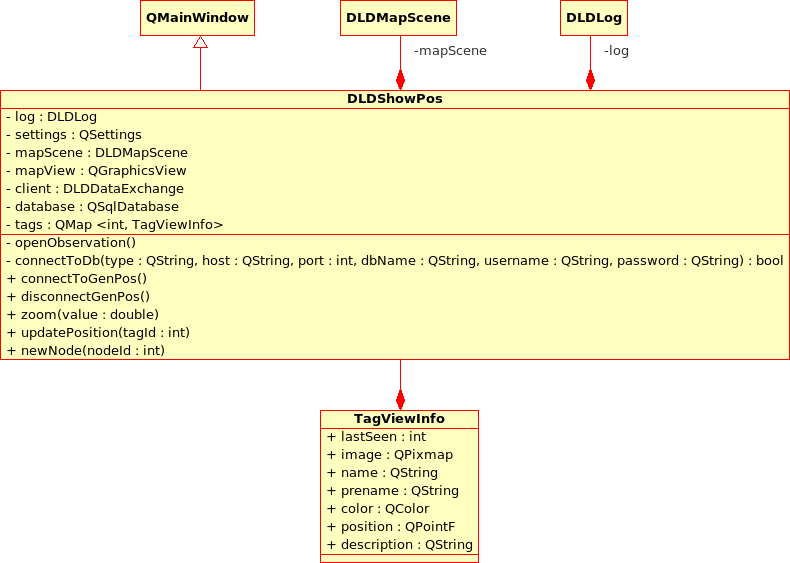
\includegraphics[scale=0.5]{UMLDiagrams/dldShowPos.png}
     \caption{UML class diagram of the Show position of a person application}
     \label{fg:projectModularization:showPos}
    \end{staticFigure}

%%%%%%%%%%%%%%%%%%%%%%%%%%%%%%%%%%%%%%%%%%%%%%%%%%%%%%%
%%%%%% MUSIC FOLLOWS YOU ADMINISTRATION INTERFACE %%%%%%
%%%%%%%%%%%%%%%%%%%%%%%%%%%%%%%%%%%%%%%%%%%%%%%%%%%%%%%
  \section{Optional application - Music follows you administration interface}
   \label{sec:design:MFUAdmin}
   This interface will be used to administrate each user of the music follows you (MFU) system. Each user has a personal login to the system and has the ability to change its zones and playlists. The administrator has the abilities to create, change, delete users and their settings.
   
   \subsection{Functionalities}
   \begin{enumerate}
    \item Administrator
       \begin{itemize}
        \item Administrate the paths from which the users can choose their songs.
        \item Administrate user (create, change, delete).
        \item Administrate zones (create, change, delete).
        \item Giving zone priorities to users.
        \item All options a user is having for itself, but the administrator has the ability to change those for each user seperatly
       \end{itemize}
    \item User
       \begin{itemize}
        \item Administrate playlists (create, change, delete).
        \item Administrate zones (create, change, delete).
        \item Select current play-mode.
        \item Select current play-list.
       \end{itemize}
   \end{enumerate}

   \subsection{Incoming data}
    \begin{itemize}
     \item User name and information by the administrator
     \item Zone information by the administrator
     \item Play-list information by the user
     \item Zone information by the user
     \item Current selections by the user
    \end{itemize}

   \subsection{Outgoing data}
    \begin{itemize}
     \item Persistent stored data in a database with all the necessary information regarding the user
    \end{itemize}

   \subsection{UML Class Diagram}
    There is no further planning for this module done, until the project has some spare time to actually do the optional tasks.

%%%%%%%%%%%%%%%%%%%%%%%%%%%%%%%%%%%%
%%%%%%   MUSIC FOLLOWS YOU    %%%%%%
%%%%%%%%%%%%%%%%%%%%%%%%%%%%%%%%%%%%
  \section{Optional application - Music follows you}
   \label{sec:design:MFU}
   The music follows you (MFU) application will provide another use of a domestic location detection which can be used to enhance the daily life. Its basic function is to let music follow a user through an environment. It will also provide the functionality to play music if a user enters a specific zone.

   An example for the first case is an audio stream that follows a person through a flat. In detail this means if a person leaves room A and enters room B the server will recognise this and then will fade out the stream to room A and start to stream to room B. To use this properly the flat has to provide an infrastructure for this, like a computer or other device that is capable of receiving an audio stream in every room/zone where the person wants to hear music.

   An example for the second case can be a museum with automated audio commentaries on the different exhibits. Each exhibit will get its own zone and as soon as a person or a group enters the zone an audio commentary will be played. A system like this would enable a museum to provide more than just a tour in a few languages. The person or group just have to register at entrance say which language is wanted and then walk on with a tag.

   \subsection{Functionalities}
    \begin{itemize}
     \item Stream different playlists to different positions
     \item Prioritise if two tags are in one zone
     \item Provide different modes (music follows you, one play-list per zone)
    \end{itemize}

   \subsection{Incoming data}
    \begin{itemize}
     \item map package containing the zone information (see section \ref{sec:design:createMapAppl})
     \item position data (see section \ref{sec:design:generatePositionDaemon})
    \end{itemize}

   \subsection{Outgoing data}
    \begin{itemize}
     \item several sound streams to several zones
    \end{itemize}

   \subsection{UML Class Diagram}
    There is no further planning for this module done, until the project has some spare time to actually do the optional tasks.

%%%%%%%%%%%%%%%%%%%%%%%%%%%%%%%
%%%%%%   COMMON CLASS    %%%%%%
%%%%%%%%%%%%%%%%%%%%%%%%%%%%%%%
  \section{Common classes}
   This section deals with classes that are used by several of the above mentioned classes.
% OB Config
   \subsection{OpenBeacon Node Communication Class}
    This class, which will be used by the ``gain data daemon''(see \ref{sec:design:gainDaemon}) as well as the ``configure OpenBeacon application'' (see \ref{sec:design:OBConfig}), provides methods that will support an easy way of communication with the OpenBeacon nodes

    \subsubsection{UML Class Diagram}
     \begin{staticFigure}
      \centering
      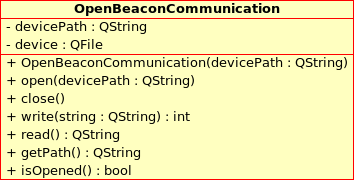
\includegraphics[scale=0.7]{UMLDiagrams/OpenBeaconCommunication.png}
      \caption{UML class diagram of the OpenBeacon Node Communication Class}
      \label{fg:projectModularization:obCommunication}
     \end{staticFigure}

    \subsubsection{Functionalities}
     This class provides all basic functionalities a device needs: open, close, read and write.

% Data exchange class
   \subsection{Data Exchange Class}
    \label{sec:design:dataExchange}
    This class provides methods for the interprocess communication. This can be achieved by using the D-Bus or the SSL strategy. If the class is used as a server then both might be used to provide data for the clients, if it is used as a client then only one strategy at a time is allowed to be used (this will prevent information collisions).

    The SSL version of the data exchange class is an optional part. At first the project has to run with D-Bus and afterwards the SSL strategy implementation should be added (if the time permits it).

    \subsubsection{UML Class Diagram}
    \begin{staticFigure}
     \centering
     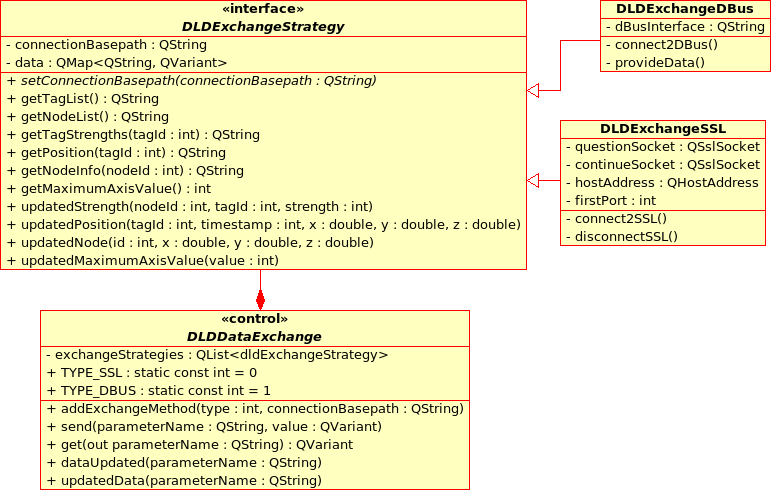
\includegraphics[scale=0.55]{UMLDiagrams/dldDataExchange.png}
     \caption{UML class diagram of the Data Exchange Class}
     \label{fg:projectModularization:dataExchange}
    \end{staticFigure}

    \subsubsection{Functionalities}
     \begin{itemize}
      \item build up SSL connection to a server or client
      \item create a D-Bus connection
      \item send data to one of the connections (or to both if it is a server)
      \item receive data from the connections
      \item store all send/received data in a map
     \end{itemize}

% Logging class
   \subsection{Log Class}
    \label{sec:design:log}
    The log class provides a set of methods to offer an easy logging facility. The log class will be used by every daemon or application.

    \subsubsection{UML Class Diagram}
     \begin{staticFigure}
      \centering
      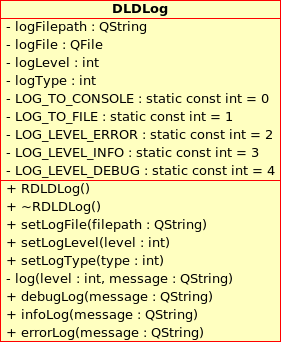
\includegraphics[scale=0.6]{UMLDiagrams/dldLog.png}
      \caption{UML class diagram of the Log Class}
      \label{fg:projectModularization:log}
     \end{staticFigure}

    \subsubsection{Functionalities}
     \begin{itemize}
      \item Log to console or file
      \item Different log levels
      \item Different files for each log levels
     \end{itemize}

% Map class
   \subsection{Optional - Map Classes}
    \label{sec:design:map}
    The map classes provide methods to handle the full map package and a map scene. A map package consists of a map description file and an image of the drawn map, both compressed into one file. The Map class will be used by the ``generate position daemon'' (see section \ref{sec:design:generatePositionDaemon}), the ``map scene'' class and any other class that needs the information of a map for saving or reading. The map scene class is a derivation of the map package class and enhances it by some scene specific features. Those features can be used to display the map in applications like the ``map generation application'' (see section  \ref{sec:design:createMapAppl}) or the ``show position of person'' application (see section  \ref{sec:design:showPosition}).

    \subsubsection{UML Class Diagram - map package}
     \begin{staticFigure}
      \centering
      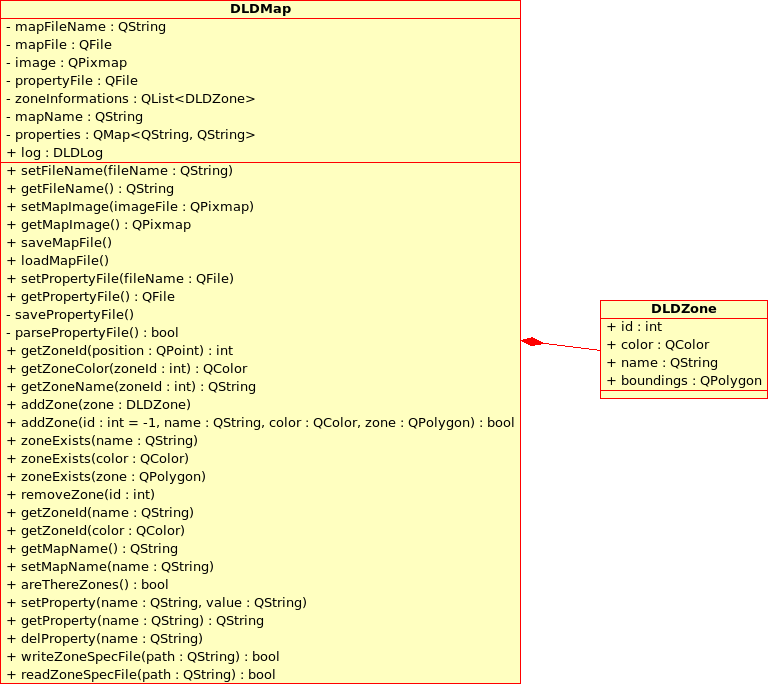
\includegraphics[scale=0.55]{UMLDiagrams/dldMap.png}
      \caption{UML class diagram of the Map Class}
      \label{fg:projectModularization:map}
     \end{staticFigure}

    \subsubsection{Functionalities - map package}
    \begin{itemize}
     \item add map image
     \item get map image
     \item add property file
     \item get property file
     \item handling of the properties
     \item open package
     \item save as package
     \item handling of the zones if there are any included
    \end{itemize}

    \subsubsection{UML Class Diagram - map scene}
     \begin{staticFigure}
      \centering
      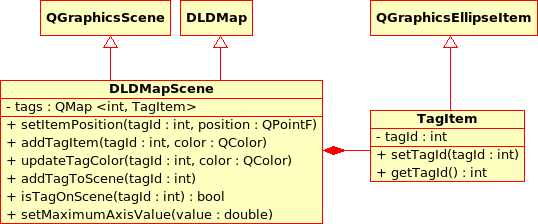
\includegraphics[scale=0.6]{UMLDiagrams/dldMapScene.png}
      \caption{UML class diagram of the Map Scene Class}
      \label{fg:projectModularization:mapScene}
     \end{staticFigure}

    \subsubsection{Functionalities - map scene}
    \begin{itemize}
     \item add tag to a scene
     \item check if tag is on the scene
     \item set the background image
     \item create a coordinate system
     \item update the position of a tag
    \end{itemize}

%%%%%%%%%%%%%%%%%%%%%%%%%%%%%%%%%%%%%%%%%%%%%
%%%  NETWORK PROTOCOL FOR SSL CONNECTIONS %%%
%%%%%%%%%%%%%%%%%%%%%%%%%%%%%%%%%%%%%%%%%%%%%
 \section{Network protocol for SSL connections}
  This section will cover the protocol and the mechanism that will be used to exchange information between the different daemons through an SSL connection. The daemons that will provide data are the ``data gain daemon'' (see section \ref{sec:design:gainDaemon}) and the ``generate position daemon'' (see section  \ref{sec:design:generatePositionDaemon}). Both provide several information regarding the positions of the tags, or persons who are wearing them, therefore the data has to be encrypted so not everyone in the net is capable of retrieving that information. The data the gain daemons provides is only interesting for the generate position daemon. The data the generate position daemon is providing on the other hand is for every application that wants to use the location data.

  To keep it as simple as possible both daemons will have the same mechanisms and methods for communicating to the connected applications. Because an asynchronous communication through TCP is not possible, the SSL communication part will use two connections. One connection is used to react on client requests and the other one is used to send regular updates in a specified interval. It should be possible to dynamically specify if both, one or none of the connections should be build up.

  \subsection*{Regular updates protocol}
   \begin{enumerate}
    \item send a raw tag strength string every N seconds. (raw tag strength string: ``tagId$|$raw$|$nodeId1=strength1$|$nodeId2=strength2$|$\dots'')
    \item send a map tag strength string every N seconds. (map tag strength string: ``tagId$|$map$|$nodeId1=strength1$|$nodeId2=strength2$|$\dots'')
    \item send a zoneUpdate if one occures. (``tagId$|$newZone'')
   \end{enumerate}

   The application which sends those strings should be capable of disabling one of the sent strength strings, so that only the needed ones are being sent. Only the generate position daemon should be able to send both, but only if it is configured that way.

  \subsection*{Reaction protocol}
   \begin{enumerate}
   \item \textbf{getTagList ()} will return a tag-list (tagId$|$tagId$|$\dots).
   \item \textbf{getTagInfo (tagId, posMode)} returns the tag strength string (``tagId$|$ nodeId1=strength1$|$nodeId2=strength2$|$\dots'') to the asked position mode.
   \item \textbf{getTagStatus (tagId)} will return the status (Gone or Seen) of the tag.
   \item \textbf{getNodeList ()} returns a list of all attached nodes
   \item \textbf{getNodeInfo (nodeId)} returns the position information of a node
   \item \textbf{getMaximumAxisValue ()} returns the maximum value of an axis in one direction
   \item \textbf{getZone (tagId)} returns the current zone of the tag
   \end{enumerate}

 \section{D-Bus Interface specification}
  This section covers the D-Bus interface specification for the gain data and generate position daemons.

  \subsection{gain data interface}
   \begin{itemize}
    \item \textbf{Service name:} org.dld.gain\\
     Service for the data gain daemon.
     \begin{enumerate}
      \item \textbf{Method:} getTagList ()\\
       returns a tag list of all seen tags so far (``tagId1$|$tagId2$|$\dots'')
      \item \textbf{Method:} getNodeList ()\\
       returns a node list of all attached nodes (``nodeId1$|$nodeId2$|$\dots'')
      \item \textbf{Method:} getTagStrengths (tagId)\\
       returns a strength string for the requested tag (``nodeId1=strength1$|$ nodeId2=strength2$|$\dots'')
      \item \textbf{Method:} getNodeInfo (nodeId)\\
       returns the coordinations of the node (``x=value$|$y=value$|$z=value'')
      \item \textbf{Method:} getMaximumAxisValue ()\\
       returns the maximum value of an axis in one direction
      \item \textbf{Signal:} updatedStrength (nodeId, tagId, strength)\\
       every time a node has a new strength available it gets sent through this signal
      \item \textbf{Signal:} updatedNode (id, x, y, z)\\
       if a new node was found its data will be sent through this signal
      \item \textbf{Signal:} updatedMaximumAxisValue (value)\\
       if the maximum axis value is changed then this signal will be emitted
     \end{enumerate}
    \item \textbf{Service name:} org.dld.genPos\\
     Service for the generate position deamon.
     \begin{enumerate}
      \item \textbf{Method:} getTagList ()\\
       see above
      \item \textbf{Method:} getPosition (tagId)\\
       returns the calculated position of the tagId
      \item \textbf{Method:} getNodeList()\\
       see above
      \item \textbf{Method:} getNodeInfo (nodeId)\\
       see above
      \item \textbf{Method:} getMaximumAxisValue ()\\
       see above
      \item \textbf{Method:} getZone (tagId)\\
       returns the zone in which the tag is currently located
      \item \textbf{Signal:} updatedPosition (tagId, timestamp, x, y, z)\\
       every time the daemon has calculated a new valid position for a tag this signal will be emitted
      \item \textbf{Signal:} updatedNode (id, x, y, z)\\
       see above
      \item \textbf{Signal:} updatedMaximumAxisValue (value)\\
       see above
      \item \textbf{Signal:} zoneChanged (tagId, newZone)\\
       this signal is emitted as soon as a tag changes from one zone to another
     \end{enumerate}
   \end{itemize}
